\label{chapter:ModelBuild}
This model build workflow
is designed to create and fine-tune a \mfus\ model, which represents a conceptual model we have of some hydrogeologic flow system, real or imaginary. \mut\ provides the link between conceptual model and \mfus\ model, and is intended to minimize the amount of time we spend building and testing it.

The first step in any workflow is to define the conceptual model, which defines the model extents, inflows and outflows and material distributions and physical properties.  To illustrate a model build, we will refer to the conceptual models developed for our existing suite of verification and illustration examples from Chapter~\ref{texfile:Examples}.

Next we need to develop a \mut\ input file, which is a plain ascii text file that you can edit with your preferred editor (e.g. Windows Notepad). \footnote{Our personal favourite editor is WinEdt (\url{https://www.winedt.com/snap.html}), which also provides a nice \LaTeX\ document development environment when coupled with the \TeX\ software package MiKTeX.  This manual was produced using these word processing tools.}
Each modflow input file name must have the extension \texttt{mut}, and a prefix of your choice. Examples of valid \mut\ input file names are \texttt{\_build.mut} or \texttt{good.mut}. Most often, the easiest approach is to copy an existing input file and modify it as required.  This helps reduce set-up time and avoid potential errors that are introduced when creating input files from scratch.

As you read along, we urge you to carry out the steps we describe as we move through the workflow.  It is good practice to copy the contents of an existing model to a new location (e.g.\ copy the folder \texttt{MUT\_Examples$\backslash$1\_VSF\_Column} to \texttt{C:$\backslash$SandBox}) and perform the actions yourself.  If you did so, your working directory would look something like this:

    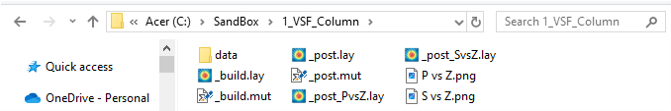
\includegraphics[width=0.4\textwidth]{3_1_vsf_column_folderinit}

In this example, there are two \mut\ input files, one for the model build called \texttt{\_build.mut}, one for post-processing called \texttt{\_post.mut} (discussed later in chapter~\ref{texfile:ModelExecution}) and a \tecplot\ layout file called \texttt{\_build.lay} used to visualize the model build results.

\mut\ tries to obtain a prefix in one of these four ways:
\begin{enumerate}
    \item \textbf{From a command line argument:} \label{commarg} At the command prompt, \mut\ checks for the presence of a command line argument.  For example, typing this:
\begin{verbatim}
    mut MyInput
\end{verbatim}
        would cause \mut\ to process the input file \texttt{MyInput.mut}.
    \item \textbf{From a prefix file:} If there is no command line argument, \mut\ checks for the presence of the file \texttt{\_mut.pfx} in the folder.  If present, \mut\ will read the prefix from it. For example, if the mut file was called \texttt{\_build.mut} then the file \texttt{mut.pfx} would have the single line \texttt{\_build}.
    \item \textbf{From the default input file:} If there is no command line argument or prefix file in the folder, \mut\ checks for the presence of the file \texttt{a.mut}.  If present in the folder, \mut\ will use it.
    \item \textbf{From the keyboard:} If none of these methods are successful, \mut\ will prompt for a prefix as shown here:

        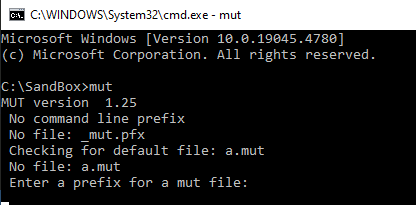
\includegraphics[width=0.6\textwidth]{3_2_mut_no_prefix}

\end{enumerate}

 In our preferred workflow, we would start a command prompt in the folder which contains the \mut\ input file as shown here:
\begin{enumerate}
    \item  Navigate to the folder in File Explorer (e.g.\ \texttt{C:$\backslash$1\_VSF\_Column\-$\backslash$SandBox}).
   \item  Click on the path in File Explorer:

        
\includegraphics[width=0.3\textwidth]{3_3_HighlightPath}

    \item  Replace the existing path with the string 'cmd':

        
\includegraphics[width=0.5\textwidth]{3_4_cmd}

    \item Press Enter/Return and you will see a command prompt rooted at the input folder e.g.:

        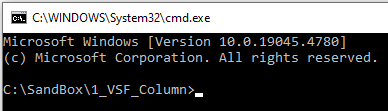
\includegraphics[width=0.4\textwidth]{3_5_cmdPrompt}

\end{enumerate}

Now run \mut\ using the input file \texttt{\_build.mut} by typing:
\begin{verbatim}
    mut _build
\end{verbatim}
As \mut\ processes the input file, note these features:
\begin{itemize}
    \item Output is written to both the screen and to the file \verb+_buildo.eco+ as execution progresses.  The first thing \mut\ writes is the version number, then the formal header, which also contains the build date.
    \item  As comment lines are stripped from the input file, they are echoed to the screen and eco file and can provide a synopsis of the input file contents.
    \item  Several new output files are created:

        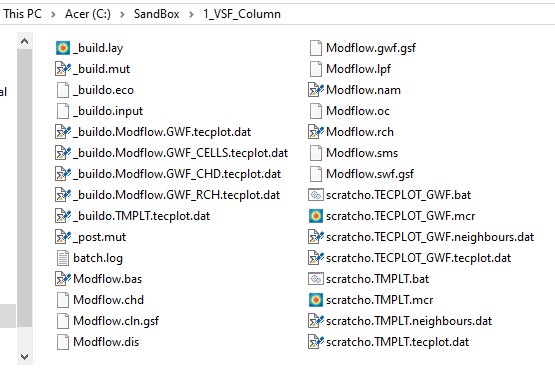
\includegraphics[width=0.8\textwidth]{3_6_buildFiles}

    \item If we start the model build prefix with the underscore character,  build output files, which have the prefix \texttt{\_buildo}, appear near the start of the list if sorted by name. The build output contains several \tecplot\ output files that are indicated by the suffix \texttt{.tecplot.dat}.
    \item Modflow model input files are written using the default prefix \texttt{Modflow}, (e.g.\ \texttt{Modflow.nam, Modflow.bas} etc.)  The prefix can be customized if desired but there are advantages to keeping this 'generic' one, such as portability of post-processing scripts or \tecplot\ layout files that follow this generic naming convention.
    \item Several scratch files (with prefix \texttt{scratcho}) are written. These are used for debugging during code development and can be ignored in most cases.
    \item \mut\ deletes previously generated output files and writes a fresh set each time it is run.  This prevents confusion that can arise when out-of-date output files are present.
        \footnote{For example, if we define a recharge boundary condition, \mut\ will create the file \texttt{\textit{prefix}o.Modflow.SWF\_RCH.Tecplot.dat} which shows the locations and recharge values assigned to Modflow cells.  If we then removed the recharge condition from the input file, but did not delete this output file, we may assume the recharge condition still applies.}
    \item If the run is successful the last line written will be \texttt{Normal exit}, otherwise an error message will be given.
\end{itemize}


If you open the file \texttt{\_build.mut} in your preferred text editor and you will see the first couple of lines are comments describing the problem:
\squish
\begin{verbatim}
    ! Examples\1_VSF_Column:
    !   A modflow project of a 1D column generated from a simple 2d rectangular mesh
\end{verbatim}
Comments begin with an exclamation point character: !\hspace{.1in}.  \mut\ creates a  clean copy of the input file called \textit{prefix}\verb+o.input+ by removing all comment lines, then processes that file to build the model. The cleaned input file contains \mut\ instructions, which may require data in the form of numbers (e.g.\ parameter values) or alphanumeric strings (e.g.\ file names).

The first instruction in the input file begins the model build:

\ins{build modflow usg}
    {This subtask has instructions that are used to define the components of the \mfus\ model such as:
     \begin{itemize}
        \item Units of length and time
        \item Numerical model meshes
        \item Material properties
        \item Boundary conditions
        \item Solver parameters
        \item Timestepping,stress periods and output control
    \end{itemize}
    Subtasks have their own unique set of instructions, which are read and processed until an \textsf{end} instruction is encountered.  We suggest appending the subtask name to the \textsf{end} instruction, which makes debugging easier when subtasks are nested:

    {\Large \sf end build modflow usg}
    }

We will use the formatting convention shown above when documenting new instructions:
\begin{itemize}
  \item Heavy upper and lower lines frame the instruction documentation.
  \item The instruction name is presented in a large sans-serif font.
  \item Data inputs, if required, are presented and described in a numbered list.
  \item General notes about instruction usage are presented.
  \item In the case of a subtask instruction, a suggested \textsf{end} instruction is presented.  The first three non-blank characters must be the string 'end', but the rest is optional.
\end{itemize}

